\chapter{Metadata Visualization}
\graphicspath{{figs/03-visualization/}}
\label{chapter:metadata-visualization}

Among the presented tools in chapter \ref{chapter:background}, MONTRA was our go-to mainly because of its data source-centric approach.
Also, no real data is shown here, only metadata is handled within the platform, however, the still allows impose access permissions at several levels.

This chapter will be detailed the key concepts of the MONTRA framework and its internal data model.
After this, there will be presented a refactoring process that was done to the platform, with its improvements and flaws fixed.

\section{MONTRA}

%\begin{itemize}
%    \item O que é o montra e o seu estado atual
%    \item explicar de maneira mais aprefundada a paltaforma, realçando partes que devem ser alteradas ou que não estão corretas
%\end{itemize}

Originally, the MONTRA framework was developed by the Bioinformatics team of the Institute of Electronics and Informatics Engineering of Aveiro associated with the \gls{emif} project with the goal to develop a common patient health information framework with emphasis on the research topics of Obesity and its metabolic complications and Markers for the development of Alzheimer's disease and other dementias.
The code is publicly available on github\footnote{https://github.com/bioinformatics-ua/montra}, whereby its development started at the beginning of 2013 and ended in the middle of 2018.
After this date, at the end of 2018, the framework started being used by the \gls{ehden} project, to develop a portal to allow discovery and analysis of health data of a federated network of data sources standardized to the \gls{omop} common data model in Europe.
Currently, the project is being developed in a private repository but has intentions to make it public after the code base is more robust and well documented.

\subsection{Communities}

In the first versions of the framework, MONTRA allowed only one level of organization related to data sources, in which they could only be separated according to their skeleton that describe their original data, which will be more detailed in the next subsection.
Newer versions created the concept of a Community.
This allows having multiple networks of data sources on the same portal, where originally the only option was to have different installations of the framework.

% TODO communities can be requested and then approved by the installation admin
% or 
% the installation can be deployed in single community mode where a community is created the first time the installation is deployed and no other communities can be created

These communities than can have different access levels:

\begin{itemize}
    \item Open: Does not require membership. Any user can access the data sources of this community
    \item Public: Does not require a membership however, the user needs to accept a set of terms and conditions before being able to access the data sources
    \item Moderated: A user has to request the community managers for approval
    \item Invitation: Users can only access and see the community by invite and subsequent approval
\end{itemize}

\subsection*{Plugins}
The concept of Community also allows customization at that level, affecting only sections within that given community.
One example of such customization are plugins
% TODO

\subsection{Questionnaires}

%\begin{itemize}
%    \item questions
%    \item tipo de questoes
%\end{itemize}

As the data from different data sources is highly heterogeneous, MONTRA ensures that the data inserted within a given community follow a common structure.
This structure is called a skeleton, which is represented in a form of a questionnaire with a set of questions, which can then be grouped in sections called Question Sets.
It represents a set of metadata that betters describes the original data of data sources that need to remain private.
The skeleton schema can easily be defined through a spreadsheet, which will be more detailed on subsection \ref{subsection:excel}.

Next is presented the available question types which can be used to build a questionnaire for a community

\begin{longtable}[c]{|c|c|}
\hline
\textbf{Type}             & \textbf{Description}                                        \\ \hline
\endhead
choice                    & single choice (radio box)                                   \\ \hline
choice-freeform           & single choice with an open text fields                      \\ \hline
choice-multiple           & multiple choice (checkbox)                                  \\ \hline
choice-multiple-freeform  & multiple choice with and open text fields                   \\ \hline
choice-tabular            & creates a table with single or multiple choices by row      \\ \hline
choice-yesno              & single choice with yea and no choices                       \\ \hline
choice-yesnodontknow      & single choice with yes, no and don't know choices           \\ \hline
comment                   & used to separate groups of questions                        \\ \hline
custom                    & mirrors another question by its                             \\ \hline
datepicker                & field with date picker widget                               \\ \hline
email                     & text input with email validation                            \\ \hline
location                  & set of select elements to choose                            \\ \hline
numeric                   & numeric input                                               \\ \hline
open                      & text field with no validation                               \\ \hline
open-button               & text input with backend validation                          \\ \hline
open-location             & text input with autocomplete sugestions                     \\ \hline
open-multiple             & allows to record an history of a value overtime             \\ \hline
open-multiple-composition & allows to record an history of values overtime              \\ \hline
open-textfield            & same as open but a textarea html tag is used                \\ \hline
open-upload-image         & image upload                                                \\ \hline
open-validated            & text input with a regex validation                          \\ \hline
publication               & a custom widget that allows to attach a set of publications \\ \hline
range                     & allows to define a range of numeric values                  \\ \hline
sameas                    & mirrors another question by its number                      \\ \hline
timeperiod                & numeric input + select to choose numeric unit               \\ \hline
url                       & text input with url validation                              \\ \hline
\caption{All available question types that can be used to build a questionnaire}
\label{tab:my-table}\\
\end{longtable}

\subsection{Fingerprints}

%\begin{itemize}
%    \item Views
%    \item validação feita toda do lado do cliente, existindo a possiblidade de ataques xss
%    \item a validação builtin do django não está a ser usada
%\end{itemize}

A fingerprint is a name given to the set of answers to the questions of a questionnaire.
In other words, it is the metadata that betters describes the original data of the associated data source.
Data owners can start to answer the questions to build the profile of their data sources once there are communities on the platform and, these have at least a questionnaire associated.

\begin{figure}[h]
    \center
    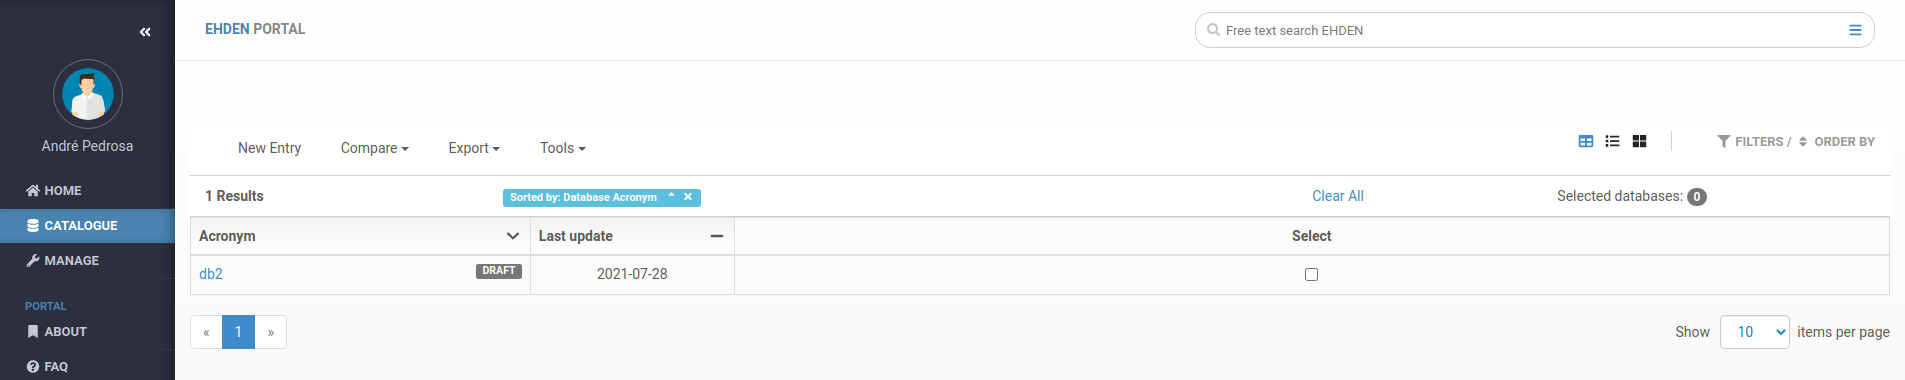
\includegraphics[width=\textwidth]{listings}
    \caption{The user interface displayed after selecting a community, which shows the list of the fingerprints of the chosen community}
    \label{fig:listings}
\end{figure}

On the list presented in figure \ref{fig:listings}, we can notice that the only fingerprint present is marked as draft.
This is a state of the fingerprint which prevents from non-ready or non-approved fingerprints won't show to the regular community users.
With this, for such users the list shows above would be empty.
Fingerprints can be published depending on the chosen settings for the community.
After the data source owners request to publish a fingerprint the framework allows to either automatically accept or require a community manger to accept it.

\subsection*{Views}

In figure \ref{fig:fingerprint-new} it is presented the user interface where a data owner can answer the questions of a questionnaire.
Each question of the questionnaire is placed under a container that can be collapsed, as is shown for question \textit{Instituition name}.
However, if multiple questions are grouped, the collapsable container will affect all questions of the group.
Besides the input widget where the data owner can insert its answers, the user also has some additional control buttons:

\begin{enumerate}
    \item Allows to Hide or Show Questions that have been answered or that are empty. Besides being an interesting feature is important to note that on the last version it does not work, as clicking on the presented options will result in no visual effect
    \item Allows to collapse or expand all questions or question groups containers
    \item Allows the data owners to set permissions at the question set level 
        \begin{itemize}
            \item Visibility: Let plugins have access to answers data
            \item Allow printing: On the fingerprints list page, showed in figure \ref{fig: listings}, there is a dropdown with tools, being the only one the "Print" tool (ref{fig:listings-tools}). However, this feature is not correctly implemented since it calls the browser's built-int printing function on the fingerprint list page, so no actual fingerprint data will be printed. This permission ends up being useless. Additionally, if a user calls the browser's print function (e.g. hitting Ctrl+P) when viewing the data of a fingerprint, the platform will not block the action.
                \begin{figure}[h]
                    \center
                    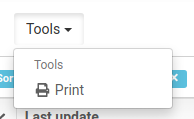
\includegraphics{listings-tools}
                    \caption{Available tools on the fingerprint selection}
                    \label{fig:listings-tools}
                \end{figure}
            \item Allow indexing: If the data owner allows indexing of the answers, which will allow for other users to find fingerprints based on the answers to a question of this specific question set.
            \item Allow exporting: If the answers to this question set can be included on the export file of a fingerprint.
        \end{itemize}
    \item Enable navigation along the question sets of the current questionnaire
    \item Permits to save or cancel all the changes made to the current question set
\end{enumerate}

\begin{figure}[h]
    \center
    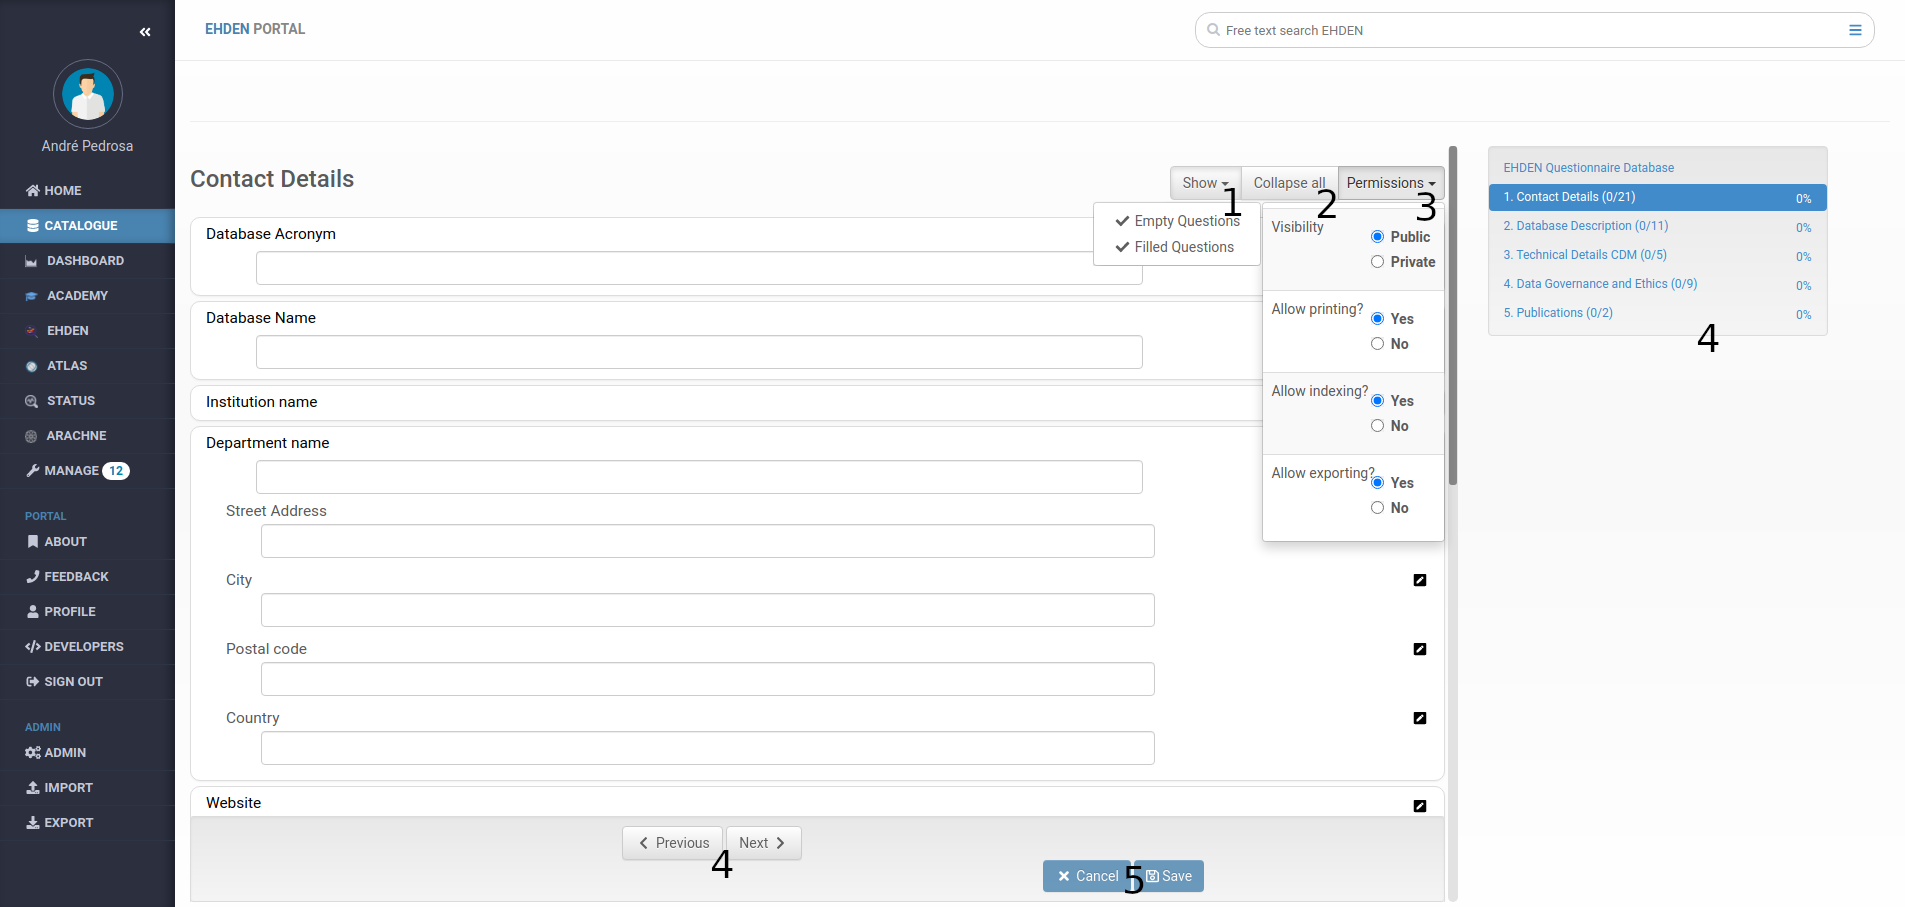
\includegraphics[width=\textwidth]{fingerprint-new}
    \caption{User interface to create a fingerprint}
    \label{fig:fingerprint-new}
\end{figure}

%% TODO grammarly

One the fingerprint is filled and published, a regular user can consult the metadata and, by default, a detailed view, similar to the create view, is presented with some different buttons:

\begin{enumerate}
    \item Database level plugins associated with this community
    \item Statistics of this fingerprint
        \begin{itemize}
            \item Progress bar + Filled: How much questions of the questionnaire were answered
            \item Hits: Number of times this fingerprint showed up on search queries
            \item Unique Views: Number of users that visited this fingerprint
        \end{itemize}
    \item Question set controls
        \begin{itemize}
            \item Summary: Allows to switch to the summary view (Figure \ref{fig:fingerprint-show-summary})
            \item Collapse \& Show: Same role as mentioned for the create view
        \end{itemize}
    \item Fingerprint control buttons
        \begin{itemize}
            \item Subscribe: Receive notifications whenever changes are made to the fingerprint answers
            \item Manage: Several fingerprint operations
                \begin{itemize}
                    \item Edit: Enter the edit mode
                    \item Share: Allows to add other users as other of the fingerprint and also to create links that enable non-logged users to consult the fingerprint
                    \item Export: Different forms of export. CSV, PDF and montra format to import on another instalations of the MONTRA framewor
                    \item Delete: Remove the fingerprint from the community
                \end{itemize}
        \end{itemize}
\end{enumerate}

\begin{figure}[h]
    \center
    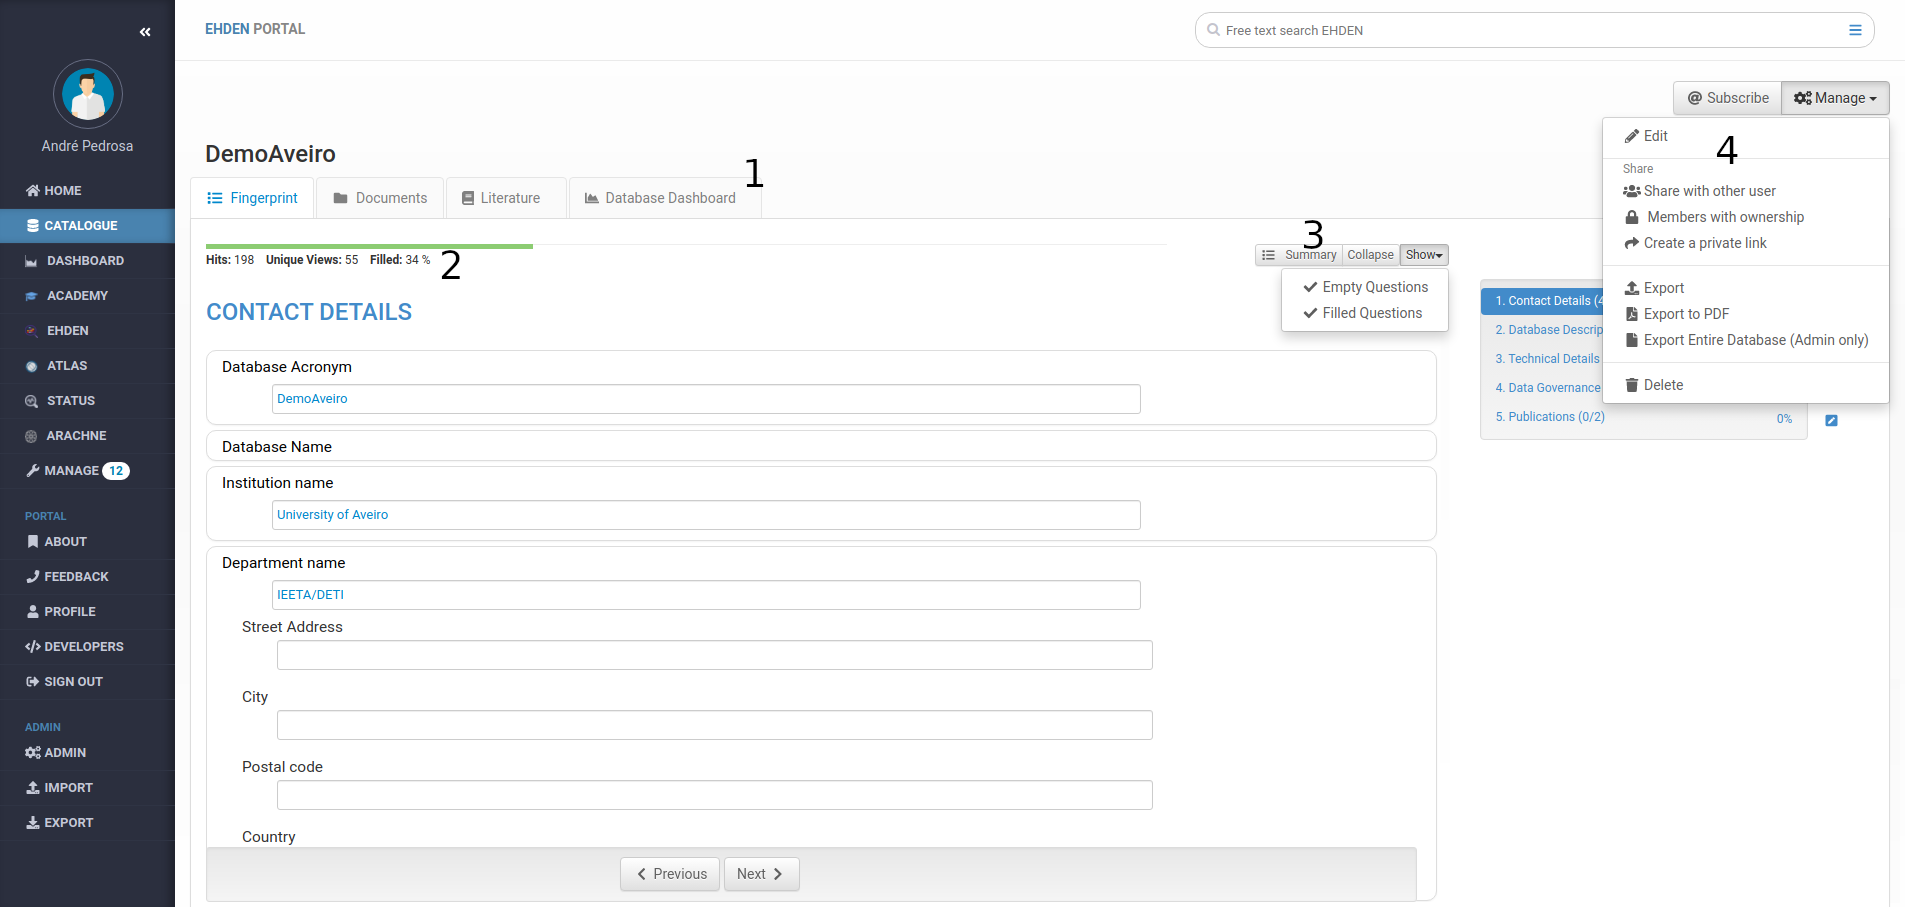
\includegraphics[width=\textwidth]{fingerprint-show-detailed}
    \caption{A detailed version user interface to view and analyze fingerprints}
    \label{fig:fingerprint-show-detailed}
\end{figure}

On the show view, if the user enters the detailed view (Figure \ref{fig:fingerprint-show-detailed}), the user is presented with a table with three columns where each row contains the question number, name and the answer given.
On this view, by hovering over an empty answer container the user can send a request to the database owner to give an answer to the specific answer.

\begin{figure}[h]
    \center
    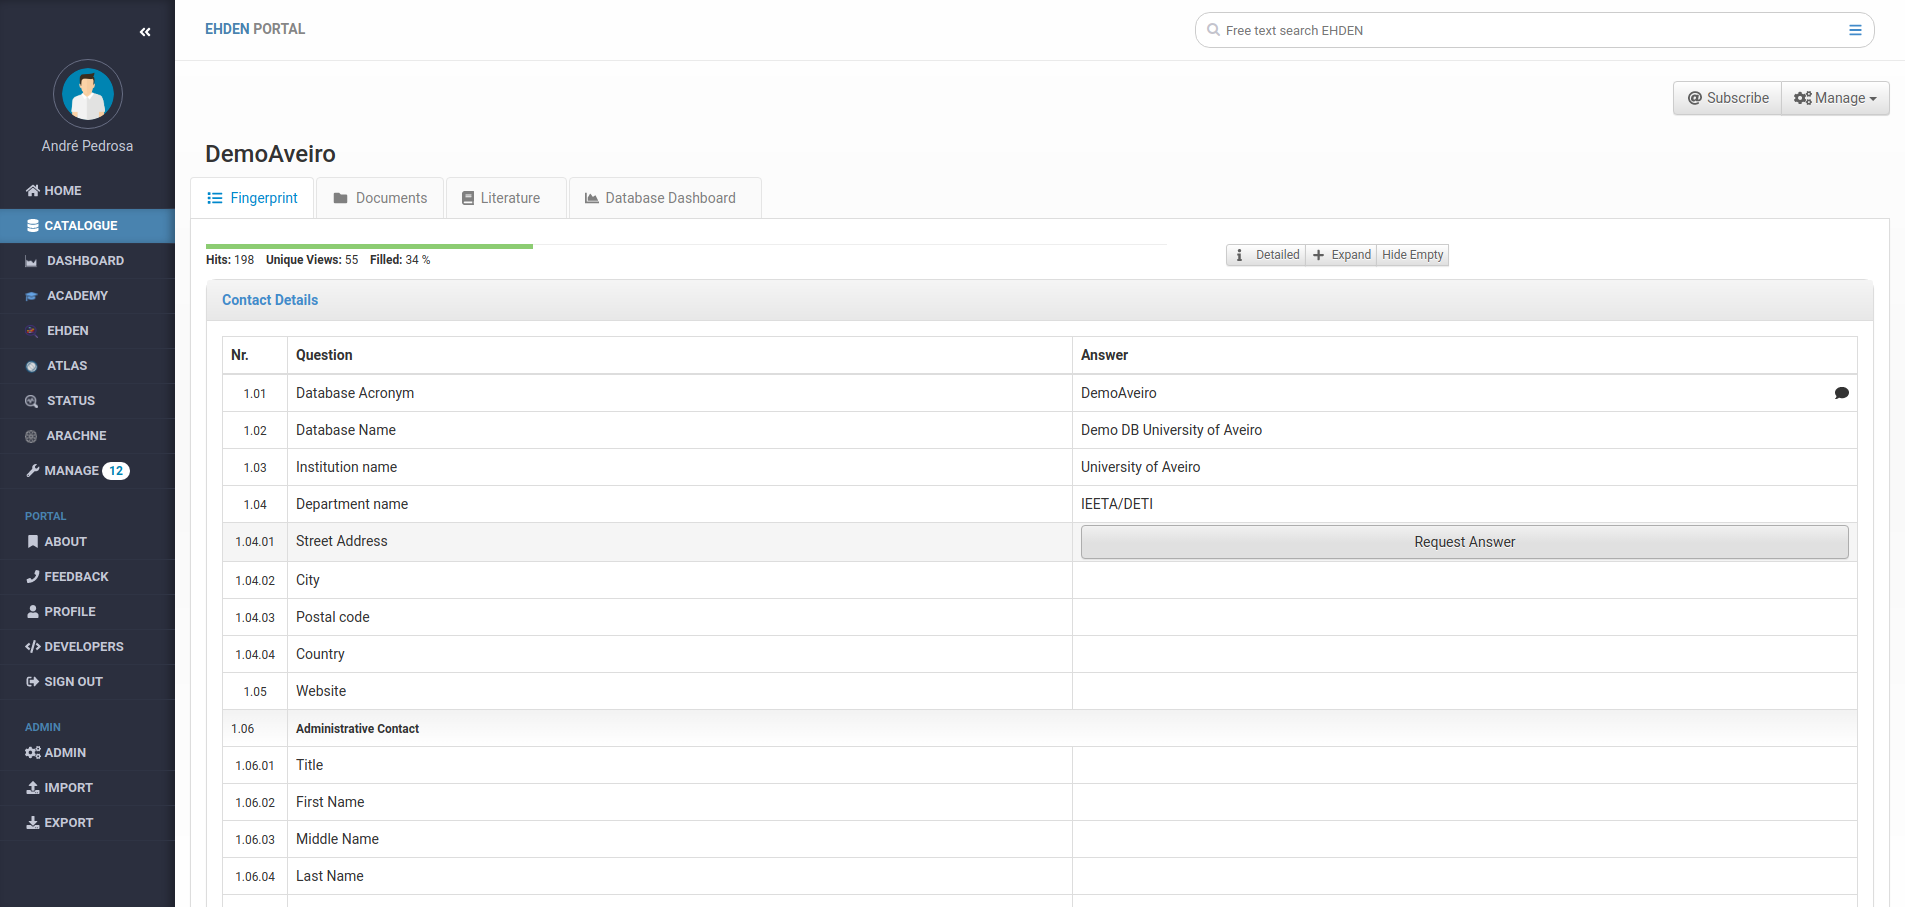
\includegraphics[width=\textwidth]{fingerprint-show-summary}
    \caption{A summary version user interface to view and analyze fingerprints}
    \label{fig:fingerprint-show-summary}
\end{figure}

The Edit view is similar to the create view, however as a checkbox on the top so the database owner can request to publish the fingerprint.

\subsection*{Input Validation}

%    \item validação feita toda do lado do cliente, existindo a possiblidade de ataques xss
%    \item a validação builtin do django não está a ser usada

\subsection{Import Questionnaires - Excel}
\label{subsection:excel}
\begin{itemize}
    \item Como os vários conceitos anteriores são mapeados para o excel
    \item Question Sets
    \item Questions
    \item Choices
    \item ...
\end{itemize}

\subsection{Data Models}
\begin{itemize}
    \item Diagrama de classes
    \item Principal intuito de cada class
    \item answers (todos os tipos guardados em texto)
\end{itemize}

\section{Refactoring}
\begin{itemize}
    \item o que necessita de, ou vai, ser alterado
\end{itemize}

\subsection{Data Models}
\begin{itemize}
    \item explicar escolha de apenas reformular apenas a apartir de determinado nivel
    \item explicar os novos modelos e de que maneiras resolvem problemas que existiam
    \item trade offs tidos em conta
    \item diagrama de classes com diferenças
    \item tipos de perguntas novos e deprecated
\end{itemize}

\subsection{Questionnaire}
\begin{itemize}
    \item UI changes
    \item consequencia da alteração do front end devido à alateração do backend
    \item passar toda a verificação para o backend, passando a usar a validação built in do Django
    \item tentar reutilizar os modulos existentes
\end{itemize}

\subsection{Excel}
\begin{itemize}
    \item mais concreto, e tem mais em conta o contexto em volta das questoes
    \item entanto é mais estenso
\end{itemize}
